% Resting objects for the shared Low Mass sanctuary. Load after
% sanctuary-scenes.tex. Every (x,y) argument is the midpoint of the lowest
% visible support/contact line, in ASGSceneUnit coordinates. These macros
% draw objects only; the calling scene owns labels, routes and occupancy.
% Insets use the existing dictionary files directly, with no asset copies.
% Trims are in bp, matching the source images' 72 dpi coordinate space.
\newcommand{\LMRestingMissalHeight}{5.5\ASGSceneUnit}
\newcommand{\LMRestingBellHeight}{4.0\ASGSceneUnit}
\newcommand{\LMRestingCruetsHeight}{3.3\ASGSceneUnit}
\newcommand{\LMRestingVeilWidth}{7.5\ASGSceneUnit}
\newcommand{\LMCoveredChaliceObjectHeight}{9\ASGSceneUnit}
\newcommand{\LMUncoveredChaliceObjectHeight}{4.0\ASGSceneUnit}
\newcommand{\LMRestingLavaboBasinWidth}{3.4\ASGSceneUnit}
\newcommand{\LMRestingLavaboTowelWidth}{3.4\ASGSceneUnit}
\newcommand{\LMRestingCommunionPlateWidth}{3\ASGSceneUnit}
\newlength{\LMObjectClipHeight}

% Gospel: the reading face turns toward picture-right and the priest.
% Epistle: the book and stand face straight forward. Neither state is made
% by mirroring the other; each retains its own inspected perspective.
\newcommand{\LMMissalObjectGOSPEL}[2]{%
  \node[anchor=south,inner sep=0pt,outer sep=0pt] at (#1,#2) {%
    
\includegraphics[height=\LMRestingMissalHeight,
      trim=90bp 176bp 2bp 287bp,clip]{liturgy/roman-rite/1962/reference/roman-sanctuary-dictionary/shared/artwork/pencil/books/RPD-FIG-books-0001-in-use-missal-on-stand-v3-alpha.png}};}
\newcommand{\LMMissalObjectEPISTLE}[2]{%
  \node[anchor=south,inner sep=0pt,outer sep=0pt] at (#1,#2) {%
    
\includegraphics[height=\LMRestingMissalHeight,
      trim=66bp 46bp 65bp 44bp,clip]{liturgy/roman-rite/1962/reference/altar-server-guides/shared/artwork/pencil/ASG-ART-068-missal-on-stand-straight.png}};}
\newcommand{\LMRestingMissal}[3]{%
  \begingroup
  \edef\LMObjectOrientation{#3}%
  \def\LMGospelOrientation{GOSPEL}%
  \def\LMEpistleOrientation{EPISTLE}%
  \ifx\LMObjectOrientation\LMGospelOrientation
    \LMMissalObjectGOSPEL{#1}{#2}%
  \else
    \ifx\LMObjectOrientation\LMEpistleOrientation
      \LMMissalObjectEPISTLE{#1}{#2}%
    \else
      \PackageError{low-mass-objects}{Unknown Missal orientation #3}{Use GOSPEL or EPISTLE.}%
    \fi
  \fi
  \endgroup}

\newcommand{\LMRestingBell}[2]{%
  \node[anchor=south,inner sep=0pt,outer sep=0pt] at (#1,#2) {%
    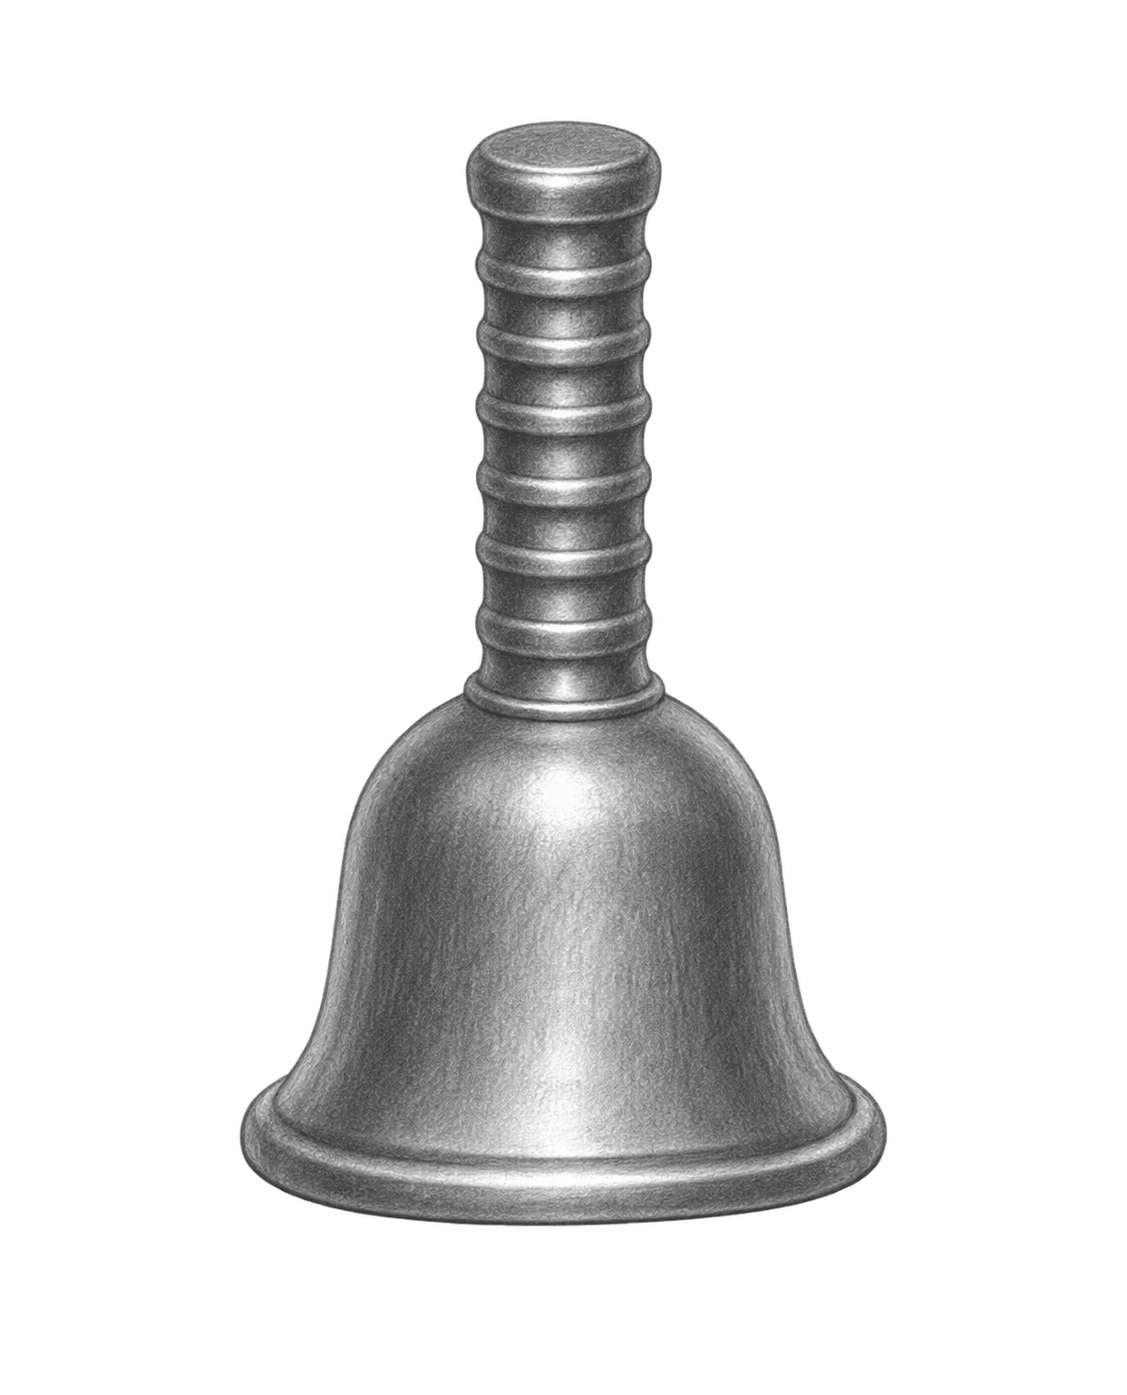
\includegraphics[height=\LMRestingBellHeight,
      trim=239bp 168bp 239bp 120bp,clip]{liturgy/roman-rite/1962/reference/altar-server-guides/shared/artwork/pencil/ASG-ART-063-single-handbell.png}};}

\newcommand{\LMRestingCruets}[2]{%
  \node[anchor=south,inner sep=0pt,outer sep=0pt] at (#1,#2) {%
    
\includegraphics[height=\LMRestingCruetsHeight,
      trim=289bp 164bp 261bp 185bp,clip]{liturgy/roman-rite/1962/reference/roman-sanctuary-dictionary/shared/artwork/pencil/RPD-FIG-service-objects-0103-paired-cruets-v2-alpha.png}};}

% The left member is assigned to wine in this model. Its generic shape does
% not identify its contents. Use this alone while Second carries the water.
\newcommand{\LMRestingWineCruet}[2]{%
  \node[anchor=south,inner sep=0pt,outer sep=0pt] at (#1,#2) {%
    
\includegraphics[height=\LMRestingCruetsHeight,
      trim=289bp 164bp 811bp 185bp,clip]{liturgy/roman-rite/1962/reference/roman-sanctuary-dictionary/shared/artwork/pencil/RPD-FIG-service-objects-0103-paired-cruets-v2-alpha.png}};}

\newcommand{\LMRestingVeil}[2]{%
  \node[anchor=south,inner sep=0pt,outer sep=0pt] at (#1,#2) {%
    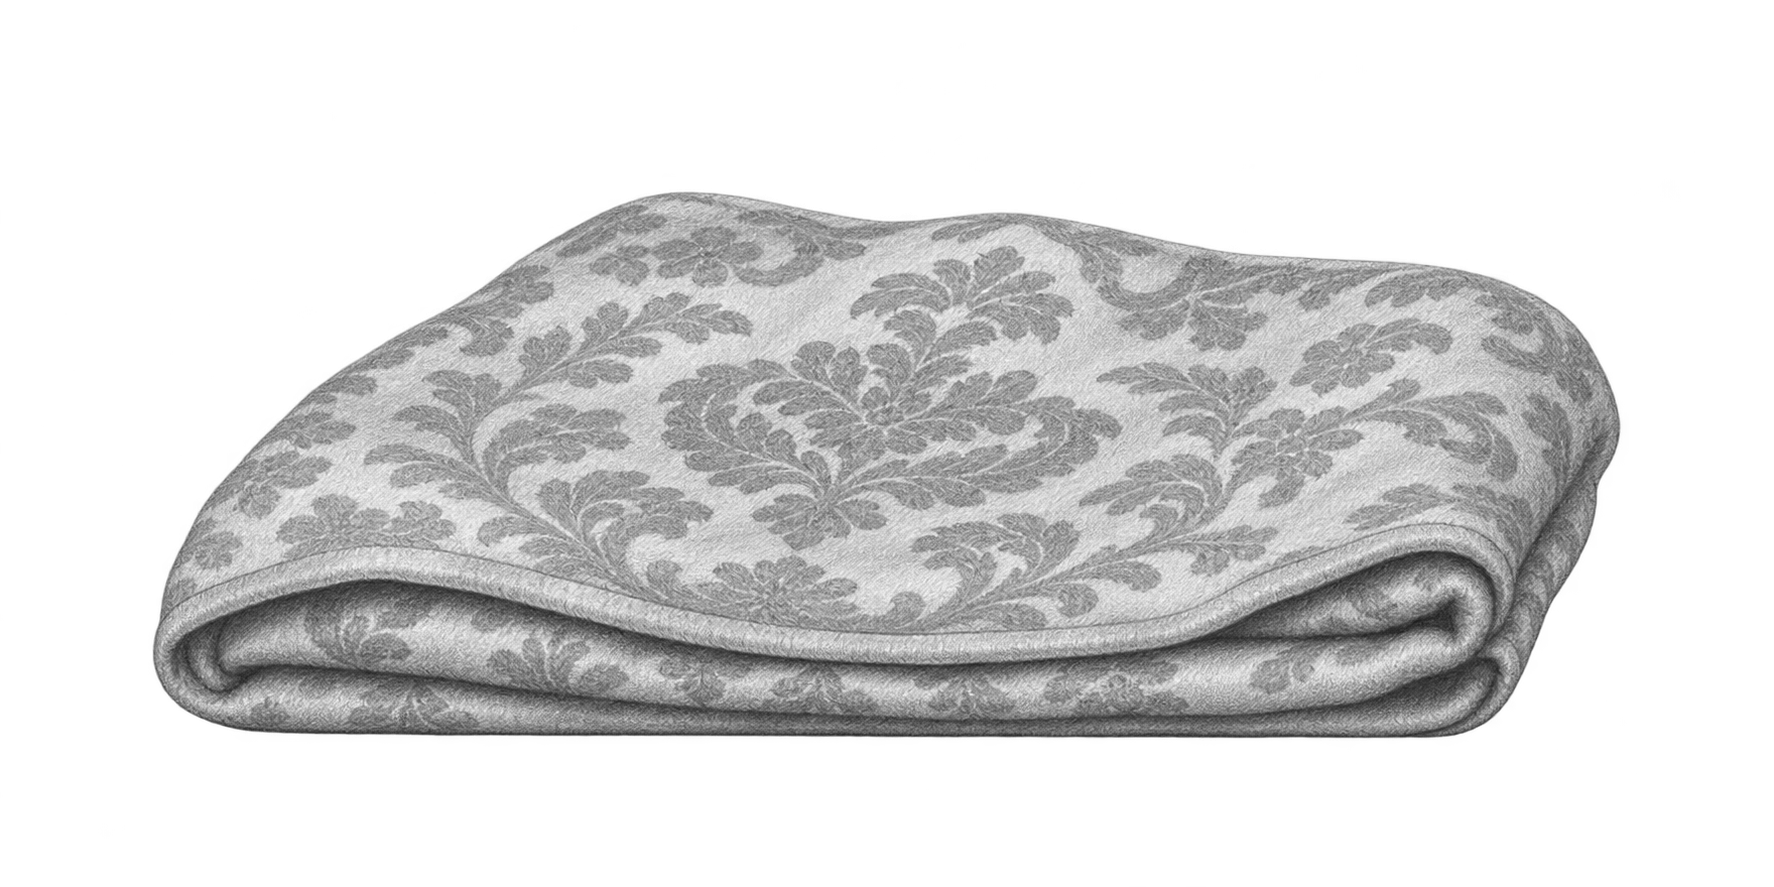
\includegraphics[width=\LMRestingVeilWidth,
      trim=152bp 148bp 153bp 191bp,clip]{liturgy/roman-rite/1962/reference/altar-server-guides/shared/artwork/pencil/ASG-ART-062-folded-chalice-veil.png}};}

% Separate crops of the dictionary's paired basin/manuterge study let the
% caller remove either object when it is being carried. The folded towel
% is the manuterge, not the purificator or folded chalice veil.
\newcommand{\LMRestingLavaboBasin}[2]{%
  \node[anchor=south,inner sep=0pt,outer sep=0pt] at (#1,#2) {%
    
\includegraphics[width=\LMRestingLavaboBasinWidth,
      trim=67bp 253bp 1034bp 323bp,clip]{liturgy/roman-rite/1962/reference/roman-sanctuary-dictionary/shared/artwork/pencil/RPD-FIG-service-objects-0106-lavabo-basin-manuterge-v2-alpha.png}};}
\newcommand{\LMRestingLavaboTowel}[2]{%
  \node[anchor=south,inner sep=0pt,outer sep=0pt] at (#1,#2) {%
    
\includegraphics[width=\LMRestingLavaboTowelWidth,
      trim=803bp 130bp 44bp 177bp,clip]{liturgy/roman-rite/1962/reference/roman-sanctuary-dictionary/shared/artwork/pencil/RPD-FIG-service-objects-0106-lavabo-basin-manuterge-v2-alpha.png}};}

% The distinct Communion plate has the one-wood-handle morphology used in
% the action study. It is not the priest's paten or the lavabo basin.
\newcommand{\LMRestingCommunionPlate}[2]{%
  \node[anchor=south,inner sep=0pt,outer sep=0pt] at (#1,#2) {%
    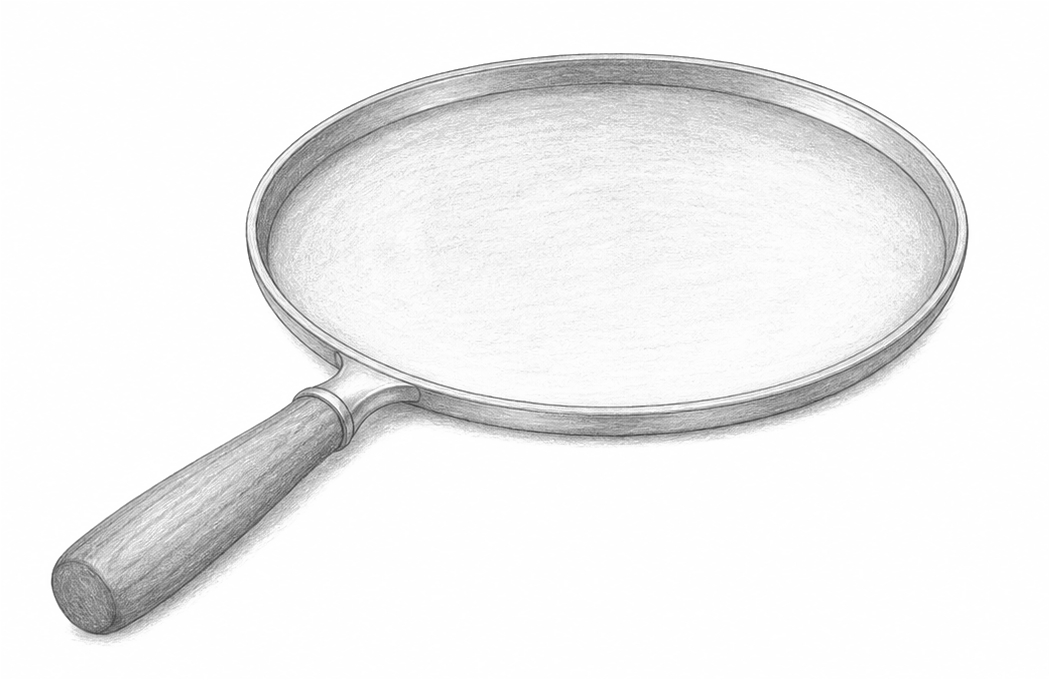
\includegraphics[width=\LMRestingCommunionPlateWidth,
      trim=50bp 44bp 81bp 50bp,clip]{liturgy/roman-rite/1962/reference/roman-sanctuary-dictionary/shared/artwork/pencil/RPD-FIG-sacred-vessels-0007-iso-communion-plate.png}};}

% The isolated round-foot vessel follows the same bowl, node and foot
% shown in the held-chalice and finger-ablution action sprites.
\newcommand{\LMUncoveredChaliceObject}[2]{%
  \node[anchor=south,inner sep=0pt,outer sep=0pt] at (#1,#2) {%
    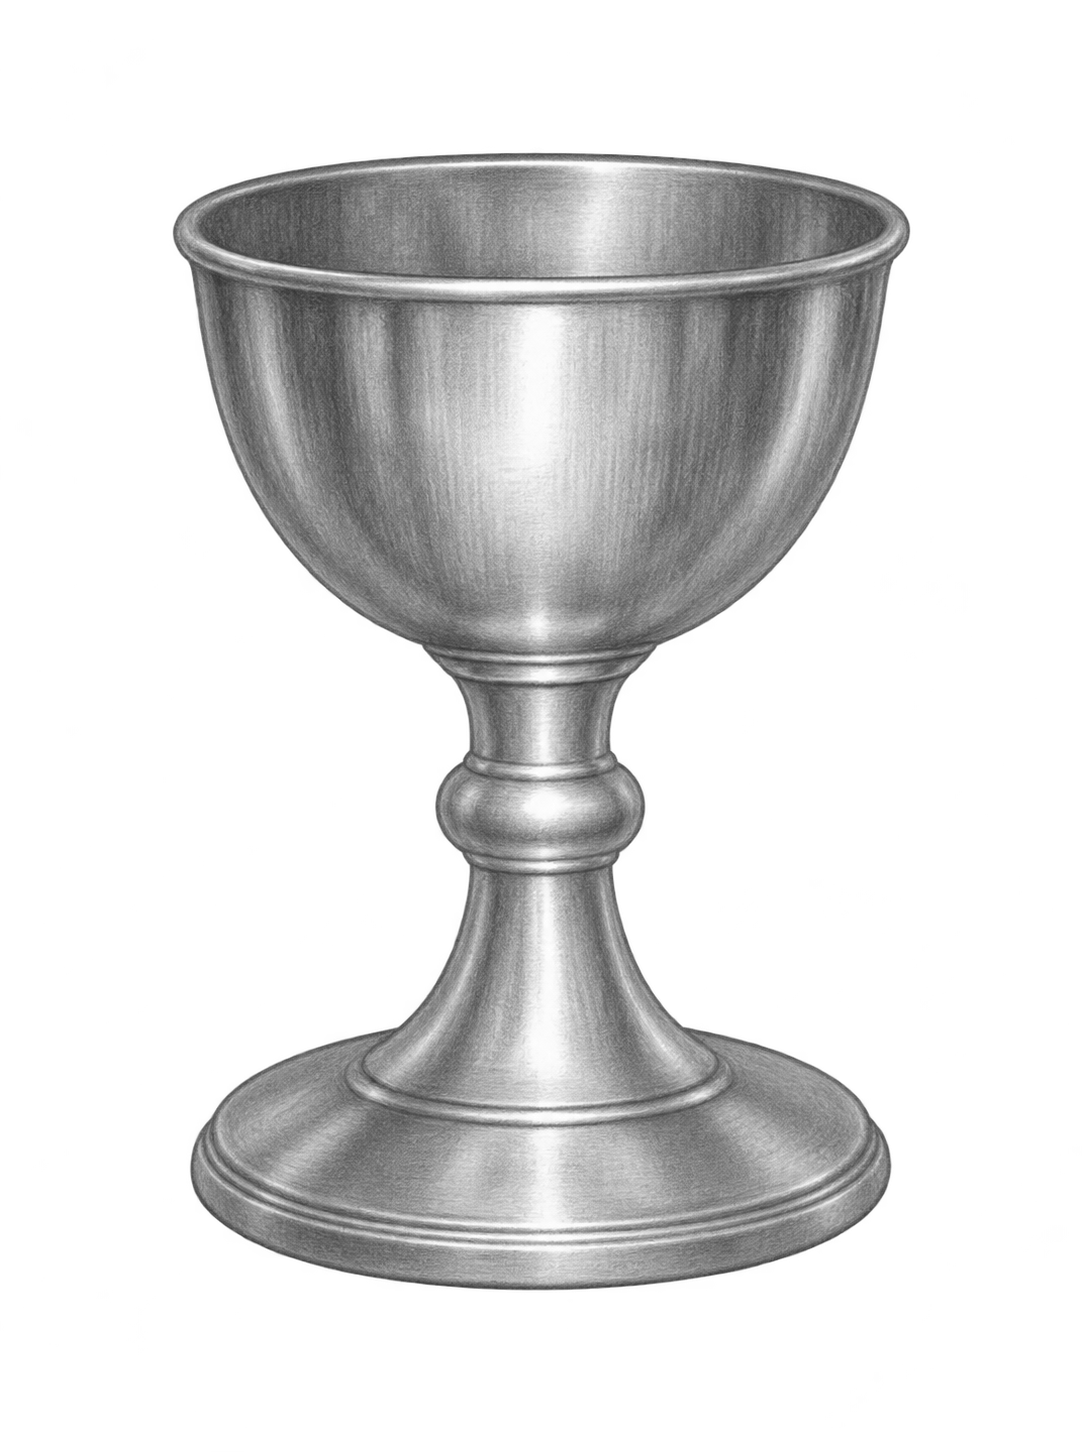
\includegraphics[height=\LMUncoveredChaliceObjectHeight,
      trim=172bp 161bp 172bp 152bp,clip]{liturgy/roman-rite/1962/reference/altar-server-guides/shared/artwork/pencil/ASG-ART-076-uncovered-chalice.png}};}

% After the offering, the pall covers the chalice before the Lavabo.
% The small plain square is a perspective recognition mark, not a claim
% about the pall's construction or dimensions. The vessel base is unchanged.
\newcommand{\LMChaliceWithPallObject}[2]{%
  \begin{scope}[shift={(#1,#2)}]
  \LMUncoveredChaliceObject{0}{0}%
  \setlength{\LMObjectClipHeight}{\LMUncoveredChaliceObjectHeight}%
  \path[fill=white,draw=black!65,line width=.2pt]
    (-.365\LMObjectClipHeight,.86\LMObjectClipHeight) --
    (.335\LMObjectClipHeight,.86\LMObjectClipHeight) --
    (.385\LMObjectClipHeight,1.015\LMObjectClipHeight) --
    (-.315\LMObjectClipHeight,1.015\LMObjectClipHeight) -- cycle;
  \end{scope}}

% Isolate only the already assembled, covered chalice at the left of the
% dictionary's formation study. The stepped clip removes the separate
% corporal in the lower-right corner without cutting the veil above it.
\newcommand{\LMCoveredChaliceObject}[2]{%
  \begin{scope}[shift={(#1,#2)}]
  \setlength{\LMObjectClipHeight}{\LMCoveredChaliceObjectHeight}%
  \clip (-.525\LMObjectClipHeight,0) --
    (.32\LMObjectClipHeight,0) --
    (.32\LMObjectClipHeight,.29\LMObjectClipHeight) --
    (.525\LMObjectClipHeight,.29\LMObjectClipHeight) --
    (.525\LMObjectClipHeight,\LMObjectClipHeight) --
    (-.525\LMObjectClipHeight,\LMObjectClipHeight) -- cycle;
  \node[anchor=south,inner sep=0pt,outer sep=0pt] at (0,0) {%
    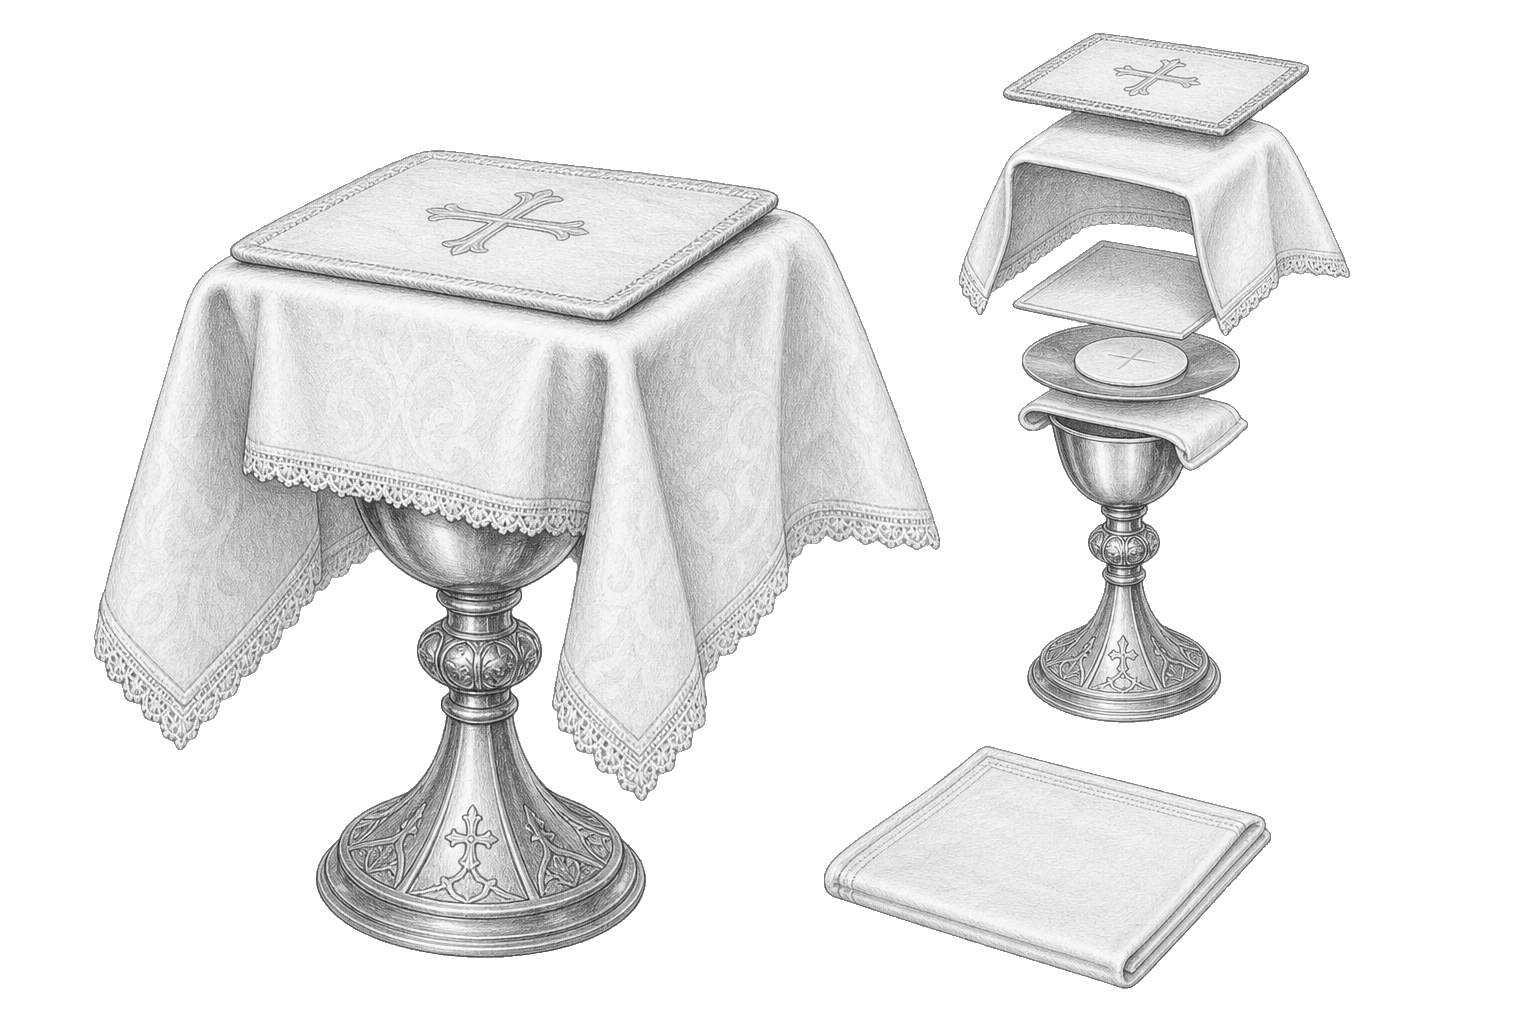
\includegraphics[height=\LMCoveredChaliceObjectHeight,
      trim=94bp 63bp 590bp 149bp,clip]{liturgy/roman-rite/1962/reference/roman-sanctuary-dictionary/shared/artwork/pencil/compositions/RPD-FIG-prepared-chalice-0001-formation-alpha.png}};
  \end{scope}}
